\section{Конструкторская часть}

В данной разделе описаны требования к программному обеспечению, разработаны схемы алгоритмов, которые будут реализованы для программного обеспечения, выполняющего реалистичное построение изображения, а также будет описаны используемые типы и структуры данных.

\subsection{Требования к программному обеспечению}

Разрабатываемое программное обеспечение должно предоставлять следующие функциональные возможности.

\begin{enumerate}[label=\arabic*.]
	\item \textbf{Построение сцены:}
	\begin{itemize}
		\item отображение тонкостенного прозрачного цилиндрического сосуда, наполненного жидкостью;
		\item отображение непрозрачного прямоугольного стержня, частично погруженного в жидкость;
		\item учет одного источника света для освещения сцены.
	\end{itemize}
	
	\item \textbf{Характеристики материалов:}
	\begin{itemize}
		\item задание характеристик материала сосуда (прозрачность, отражаемость, коэффициент преломления, цвет);
		\item задание характеристик материала жидкости (прозрачность, отражаемость, коэффициент преломления, цвет);
		\item задание характеристик материала стержня (отражаемость, цвет).
	\end{itemize}
	
	\item \textbf{Пользовательский интерфейс:} предоставление удобного графического интерфейса для изменения параметров сцены (характеристик материалов, положения источника света и камеры в сцене).
	
	\item \textbf{Рендеринг изображения:}
	\begin{itemize}
		\item построение изображения с реалистичными эффектами освещения;
		\item отображение результатов с учетом прозрачности, отражения, преломления и теней;
		\item экспорт финального изображения в стандартные графические форматы (например, PNG, JPEG).
	\end{itemize}
\end{enumerate}

\subsection{Разработка алгоритмов}

Далее будут описаны схемы алгоритмов, которые будут реализованы при разработке проргаммного обеспечения.

\subsubsection{Модель освещения Фонга}

Модель освещения Фонга, как показано на рисунке~\ref{fig:0}, включает три компонента~\cite{phong1975illumination}:

\begin{enumerate}[label=\arabic*)]
	\item \textbf{диффузное освещение} -- пропорциональное косинусу угла между нормалью поверхности и направлением света;
	\item \textbf{зеркальное освещение} -- имитирующее яркие блики, зависящие от угла между отраженным светом и направлением камеры;
	\item \textbf{фоновое освещение} -- добавляет общее освещение.
\end{enumerate}

\begin{figure}[ht!]
	\begin{center}
		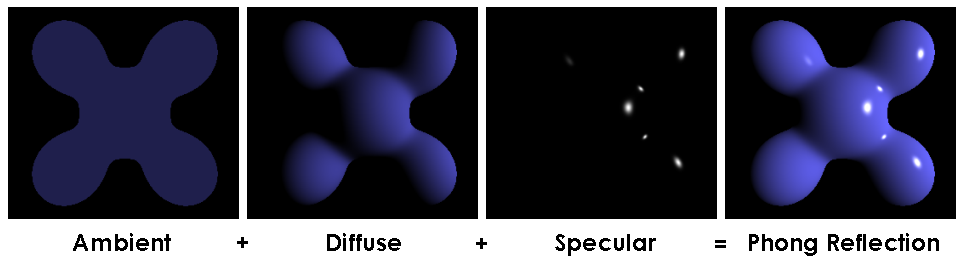
\includegraphics[scale=0.65]{img/phong.png}
	\end{center}
	\caption{Визуальная иллюстрация уравнения Фонга}
	\label{fig:0}
\end{figure}


Тогда \textbf{полное освещение} для пикселя является суммой этих трех компонентов:

\begin{equation}
	I = I_{ambient} + I_{diffuse} + I_{specular},
\end{equation}
где $I$ -- полная интенсивность освещения для пикселя;  $I_{ambient}$, $I_{diffuse}$, $I_{specular}$~-- компоненты освещения (фоновое, диффузное и зеркальное освещения, соответственно).

На рисунке~\ref{fig:phong} изображена схема алгоритма вычисления полного освещения для пикселя.

\begin{figure}[ht!]
	\begin{center}
		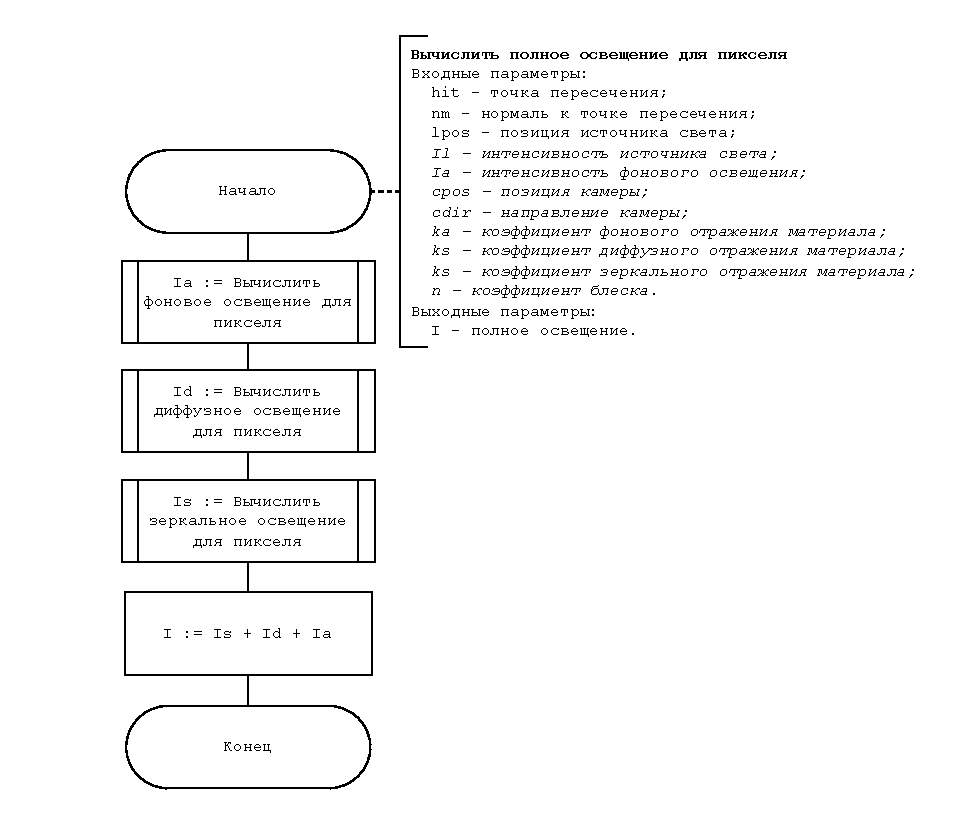
\includegraphics[scale=1.05]{diag/main-phong.pdf}
	\end{center}
	\caption{Cхема алгоритма вычисления зеркального освещения для пикселя}
	\label{fig:phong}
\end{figure}

\textbf{Фоновое освещение} можно вычислить по формуле

\begin{equation}
	I_{ambient} = k_a \cdot I_a,
\end{equation} где \( k_a \) -- коэффициент фонового освещения для материала; \( I_a \) -- интенсивность фонового света.

На рисунке~\ref{fig:phong-ambient} изображена схема алгоритма вычисления фонового освещения для пикселя.

\begin{figure}[ht!]
	\begin{center}
		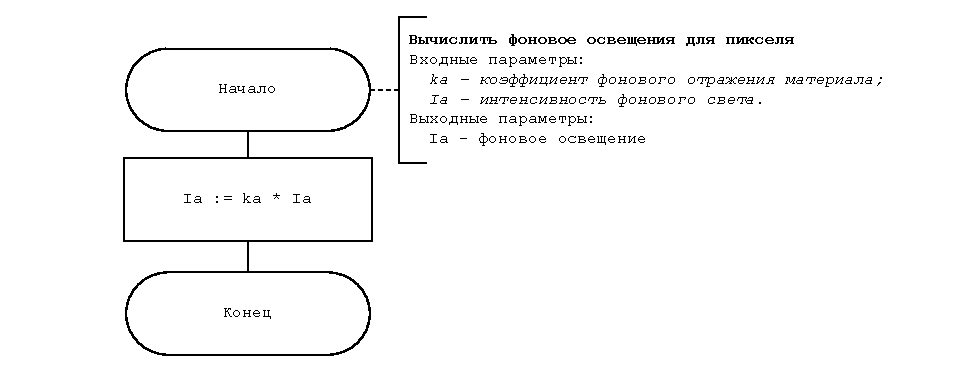
\includegraphics[scale=1.0]{diag/main-phong-ambient.pdf}
	\end{center}
	\caption{Cхема алгоритма вычисления фонового освещения для пикселя}
	\label{fig:phong-ambient}
\end{figure}

\textbf{Зеркальное освещение} можно вычислить по формуле

\begin{equation}
	I_{specular} = k_s \cdot I_L \cdot \left( \max(0, \mathbf{R} \cdot \mathbf{V}) \right)^n,
\end{equation} где:

\begin{itemize}
	\item \( k_s \) -- коэффициент зеркального отражения материала;
	\item \( \mathbf{R} = 2 \cdot (\mathbf{N} \cdot \mathbf{L}) \cdot \mathbf{N} - \mathbf{L} \) -- вектор отражения, который вычисляется как отражение вектора \( \mathbf{L} \) относительно нормали \( \mathbf{N} \);
	\item \( \mathbf{V} \) -- единичный вектор, направленный от точки пересечения луча к камере;
	\item \( n \) -- коэффициент блеска (или экспонента);
	\item \( \max(0, \mathbf{R} \cdot \mathbf{V}) \) -- эта функция гарантирует, что только те блики, которые направлены в сторону камеры, будут учтены.
\end{itemize}

На рисунке~\ref{fig:phong-spec} изображена схема алгоритма вычисления зеркального освещения для пикселя.

\newpage
\begin{figure}[ht!]
	\begin{center}
		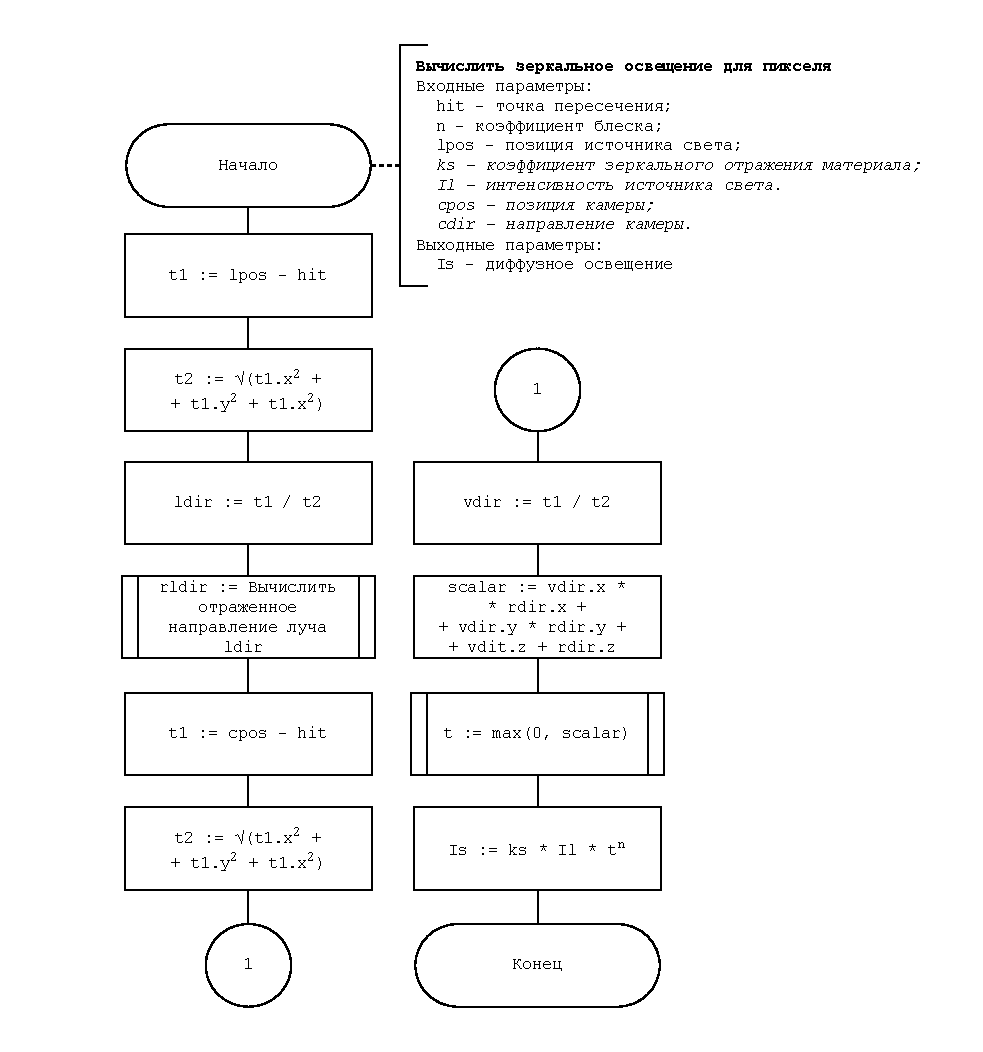
\includegraphics[scale=1.0]{diag/main-phong-specular.pdf}
	\end{center}
	\caption{Cхема алгоритма вычисления зеркального освещения для пикселя}
	\label{fig:phong-spec}
\end{figure}

\textbf{Диффузное освещение} можно вычислить по формуле

\begin{equation}
	I_{diffuse} = k_d \cdot I_L \cdot \max(0, \mathbf{N} \cdot \mathbf{L}),
\end{equation}где:
\begin{itemize}
	\item \( k_d \) — коэффициент диффузного отражения материала;
	\item \( I_L \) — интенсивность источника света;
	\item \( \mathbf{N} \) — нормаль поверхности в точке пересечения луча;
	\item \( \mathbf{L} \) — единичный вектор, направленный от точки пересечения луча к источнику света.
\end{itemize}

На рисунке~\ref{fig:phong-diff} изображена схема алгоритма вычисления диффузного освещения для пикселя.

\begin{figure}[ht!]
	\begin{center}
		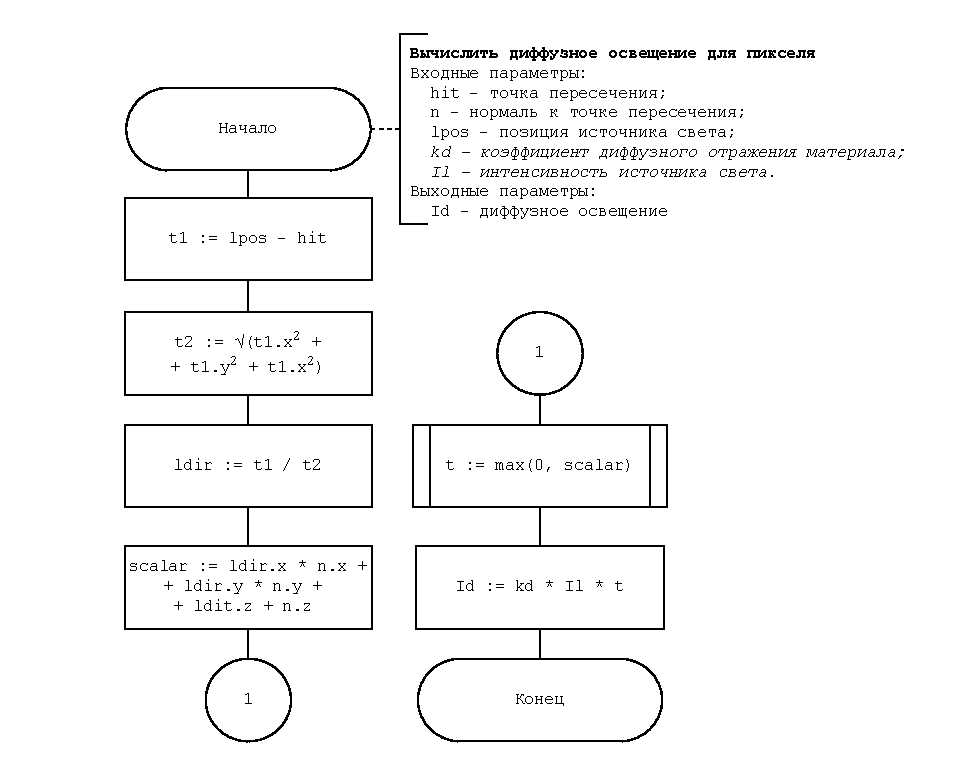
\includegraphics[scale=1.0]{diag/main-phong-diffuse.pdf}
	\end{center}
	\caption{Cхема алгоритма вычисления диффузного освещения для пикселя}
	\label{fig:phong-diff}
\end{figure}

\subsubsection{Обратная трассировка лучей}

Для разработки алгоритма обратной трассировки лучей необходимо описать, как вычисляются пересечение луча с объектами сцены, преломление и отражение луча.

\subsubsection*{Пересечение луча с объектом}

Уравнение прямой описывается следующей формулой~\cite[c.~140]{lengyel2011mathematics}.

\begin{equation}
P(t) = S + t \cdot V,
\end{equation}
где $P(t)$ -- точка на прямой, которая выражается с помощью параметра t (меняется в диапазоне от минимального до максимального значения для задания всей прямой); $V$ -- вектор направления прямой, который определяет, в каком направлении прямая распространяется от начальной точки $S$.

Тогда значение параметра $t$, соответствующее точке пересечения, например, с плоскостью \textbf{параллелепипеда}, заданным формулой~(\ref{box}), $x = r_x$, можно вычислить следующим образом~\cite[c.~143]{lengyel2011mathematics}. 

\begin{equation}
	t = \frac{r_x - S_x}{V_x},
\end{equation} при этом
координаты $y$ и $z$ точки пересечения внутри граней параллелограмма должны удовлетворять условиям:

\begin{equation}
 	0 \leq [P(t)]_y \leq r_y;	0 \leq [P(t)]_z \leq r_z.
\end{equation}

Значение параметра $t$ соответствующее точке пересечения с плоскостями параллелепипеда  $z = r_z$, $y = r_y$ вычисляется аналогично.

Уравнение~(\ref{cyl}), задающее \textbf{цилиндр}, можно привести к следующему виду~\cite[С.~145--146]{lengyel2011mathematics}:
\begin{equation}
	(V_x^2 + m^2V_y^2)t^2 + 2(S_xV_x + m^2S_yV_y)t + S_x^2 + m^2Sy^2 - r^2 = 0.
\end{equation}

Решение этого уравнение дает значение параметра $t$, где луч пересекает бесконечный цилиндр. Полученные точки пересечения должны быть проверены по $z$-координатам, чтобы удовлетворять условию:

\begin{equation}
	0 \leq z \leq h,
\end{equation}
где $h$ -- высота цилиндра.

На рисунке~\ref{fig:intc} изображена схема алгоритма нахождения точки пересечения луча с цилиндром.

\begin{figure}[ht!]
	\begin{center}
		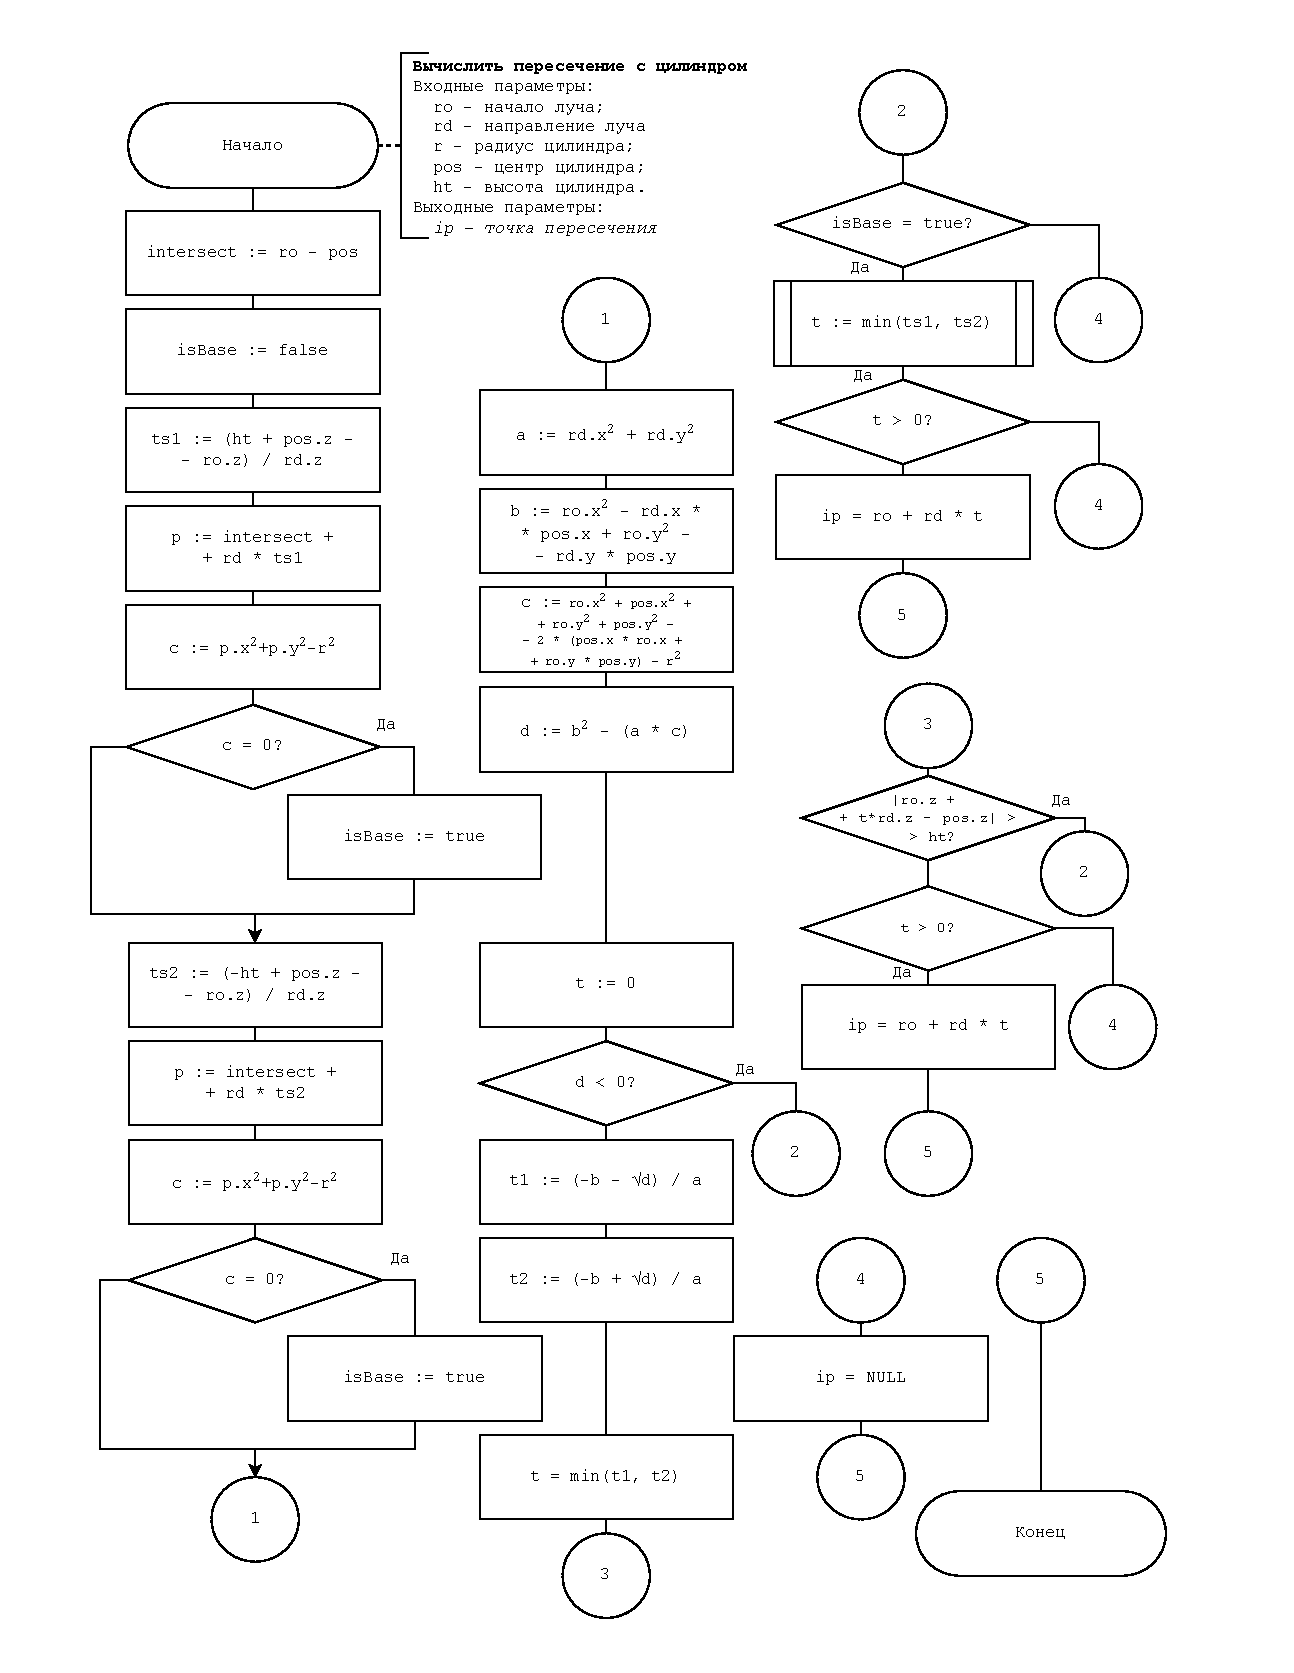
\includegraphics[scale=0.8]{diag/main-raycast-cylinder.pdf}
	\end{center}
	\caption{Cхема алгоритма нахождения точки пересечения луча с цилиндром}
	\label{fig:intc}
\end{figure}

На рисунке~\ref{fig:intb} изображена схема алгоритма нахождения точки пересечения луча с параллелепипедом.

\begin{figure}[ht!]
	\begin{center}
		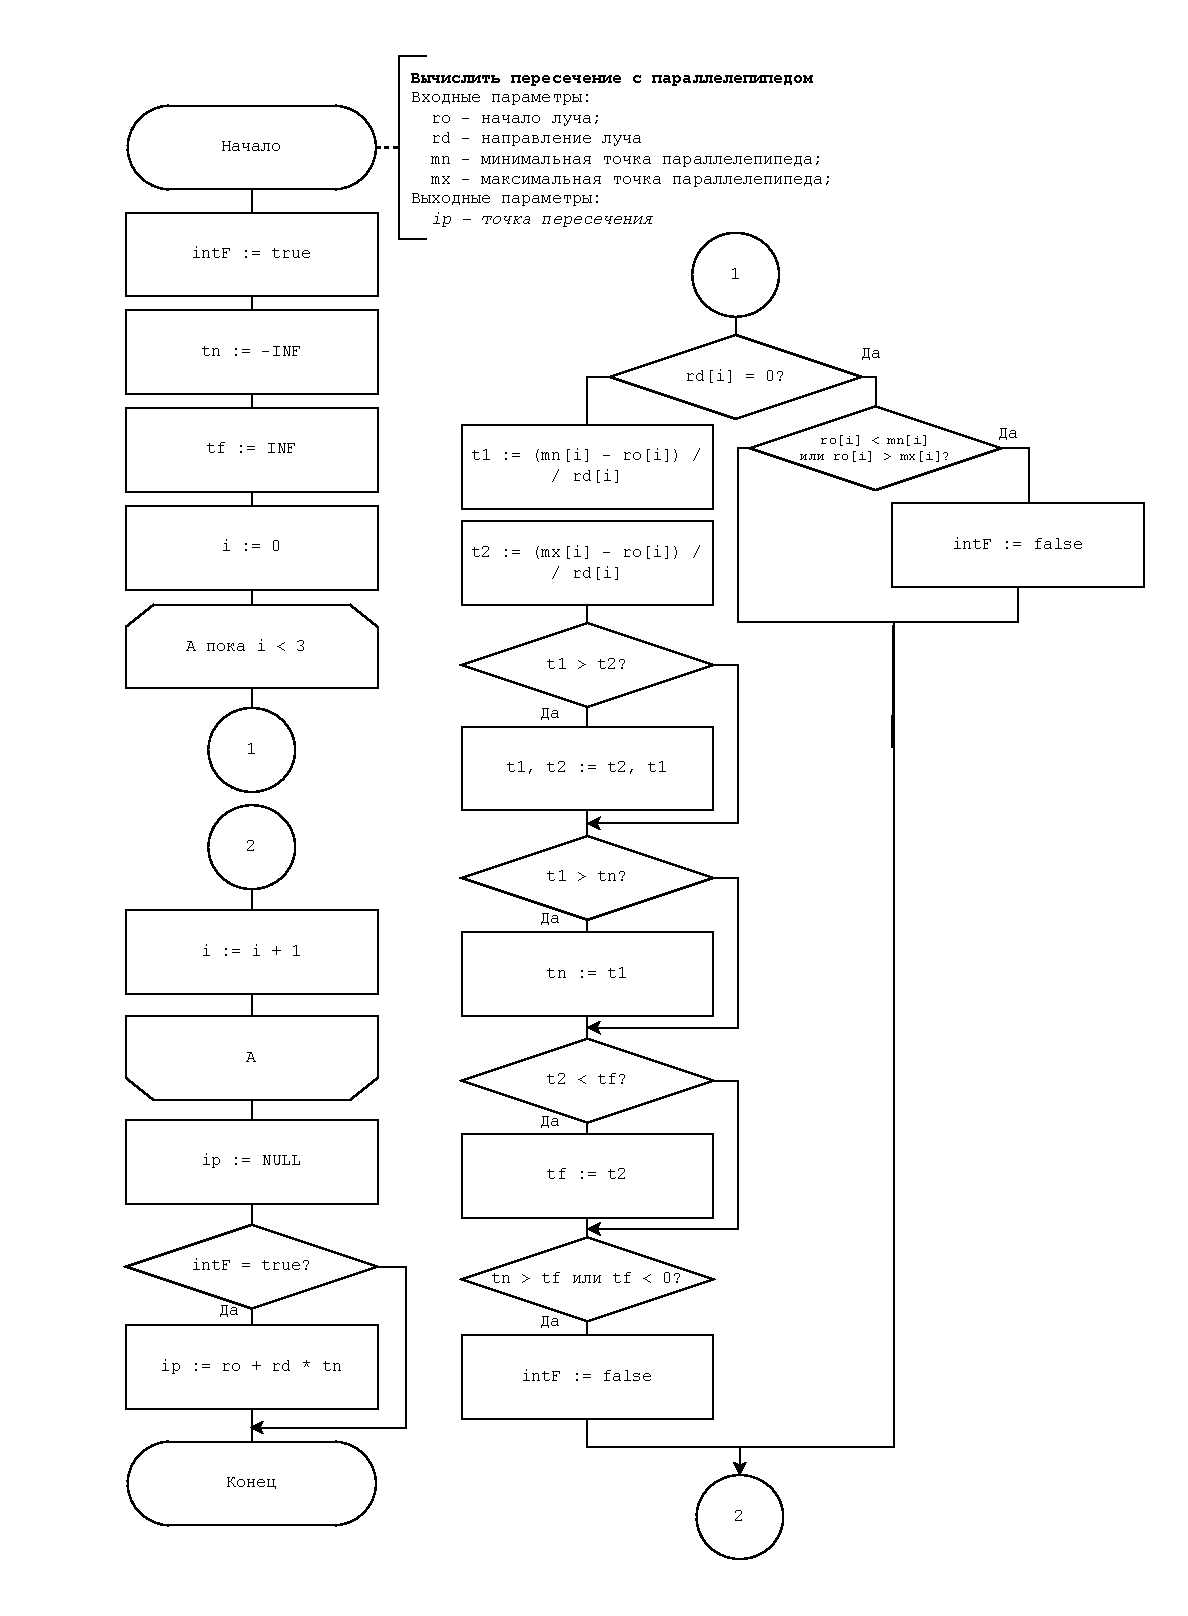
\includegraphics[scale=0.78]{diag/main-raycast-parallel.pdf}
	\end{center}
	\caption{Cхема алгоритма нахождения точки пересечения луча с параллелепипедом}
	\label{fig:intb}
\end{figure}

\subsubsection*{Отражение луча}

Направление отражения света от блестящей поверхности подчиняется правилу: угол падения равен углу отражения, как показано на рисунке~\ref{fig:1}~\cite[c.~150]{lengyel2011mathematics}.

Пусть векторы $N$ и $L$ нормализованы -- единичной длины. Тогда вектор $R$ -- направление отраженного луча, можно вычислить следующий образом:

\begin{equation}
	R = 2(N \cdot L)N - L.
\end{equation}

\begin{figure}[ht!]
	\begin{center}
		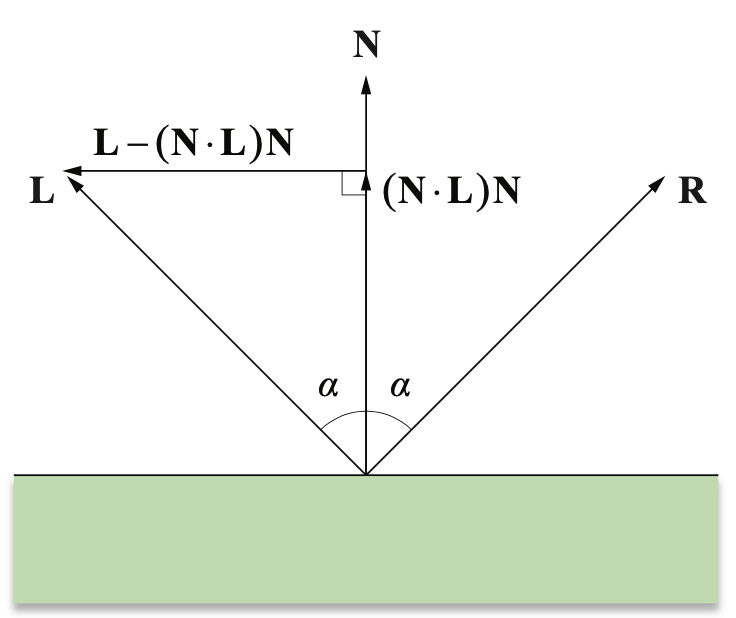
\includegraphics[scale=0.4]{img/reflection.png}
	\end{center}
	\caption{Отражение луча от поверхности~\cite[c.~150]{lengyel2011mathematics}}
	\label{fig:1}
\end{figure}

На рисунке~\ref{fig:refl} изображена схема алгоритма вычисления отраженного луча.

\begin{figure}[ht!]
	\begin{center}
		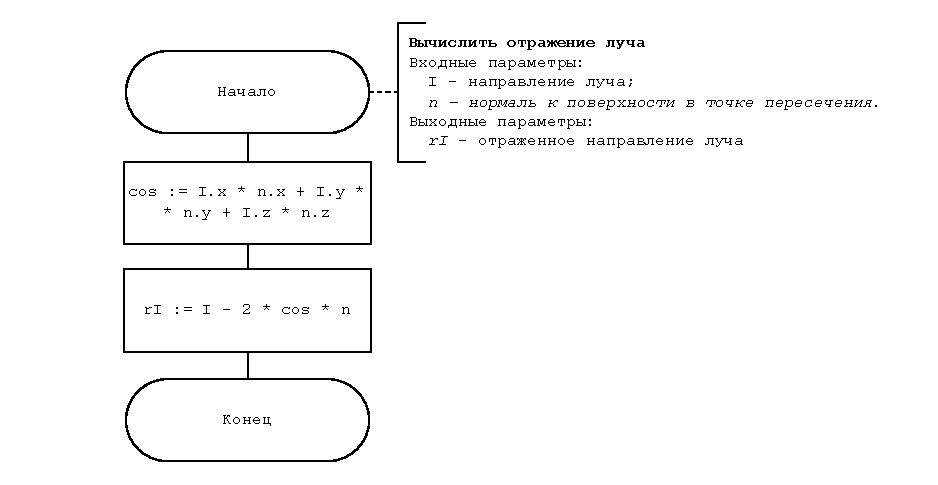
\includegraphics[scale=0.9]{diag/main-raytracing-reflect.pdf}
	\end{center}
	\caption{Схема алгоритма вычисления отражения луча от поверхности}
	\label{fig:refl}
\end{figure}

\subsubsection*{Преломление луча}

Согласно закону Снеллиуса, как показано на рисунке~\ref{fig:2}, угол падения \( \theta_L \) и угол преломления \( \theta_T \) для двух сред с показателями преломления $\eta_L$ и $\eta_T$ связаны уравнением~\cite[c.~151]{lengyel2011mathematics}:

\begin{equation}
	\eta_L \sin(\theta_L) = \eta_T \sin(\theta_T).
\end{equation}

\begin{figure}[ht!]
	\begin{center}
		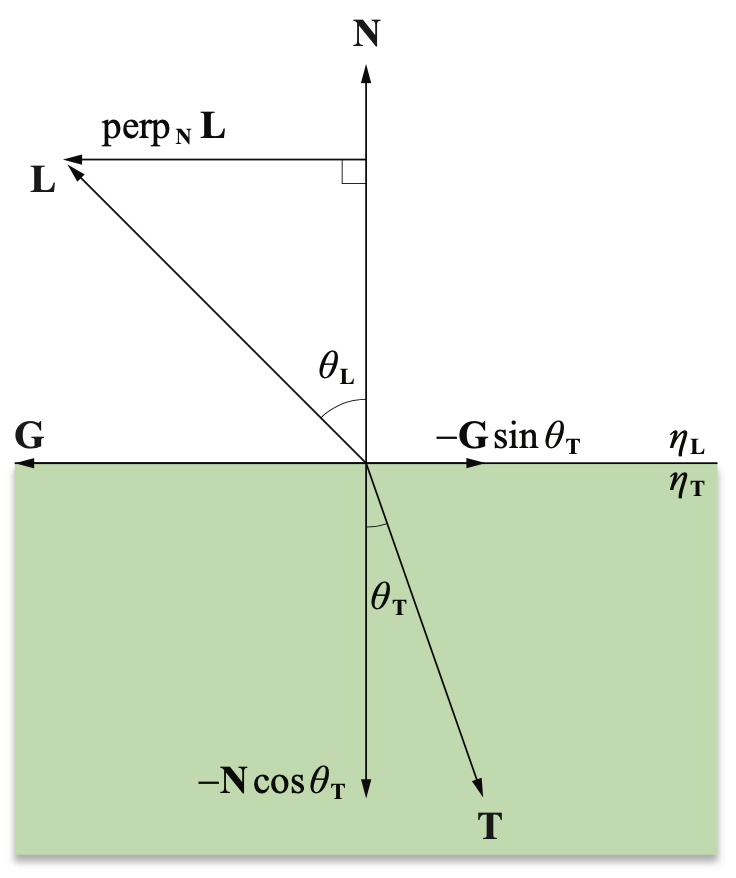
\includegraphics[scale=0.6]{img/refraction.png}
	\end{center}
	\caption{Преломление луча, на границе двух сред~\cite[c.~152]{lengyel2011mathematics}}
	\label{fig:2}
\end{figure}

Пусть векторы $N$ и $L$ нормализованы -- единичной длины. Тогда вектор $T$ -- направление преломления, можно вычислить следующий образом:

\begin{equation}
	T = \Bigg(\frac{\eta_L}{\eta_T} N \cdot L - \sqrt{1 - \frac{\eta_L^2}{\eta_T^2}[1 - (N \cdot L)^2]}\Bigg)N - \frac{\eta_L}{\eta_T}L.
\end{equation}

На рисунке~\ref{fig:refr} изображена схема алгоритма вычисления преломления луча.

\newpage
\begin{figure}[ht!]
	\begin{center}
		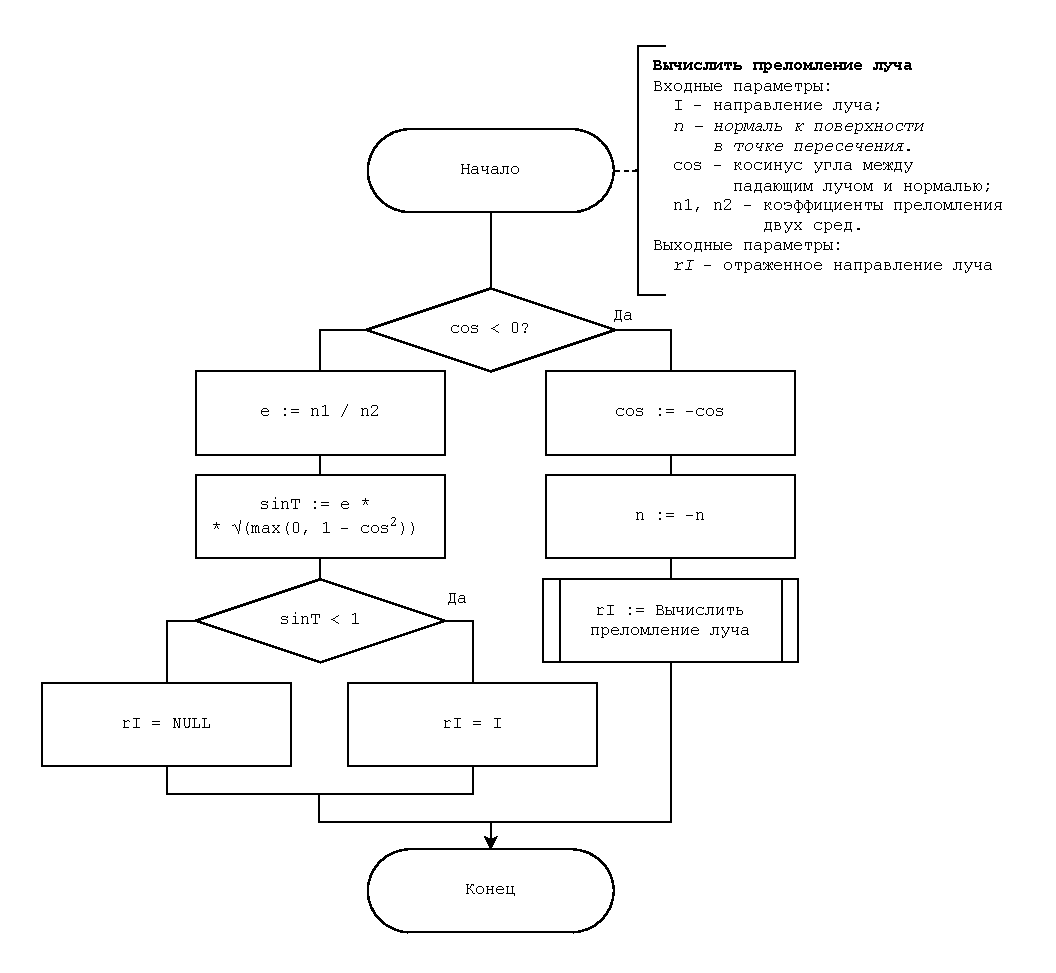
\includegraphics[scale=1]{diag/main-raytracing-refract.pdf}
	\end{center}
	\caption{Схема алгоритма вычисления преломления луча}
	\label{fig:refr}
\end{figure}

\subsubsection*{Алгоритм прямой трассировки лучей}

На рисунке~\ref{fig:pixel} изображена схема обощенного алгоритма обратной трассировки луча для вычисления цвета одного пикселя изображения.

\newpage
\begin{figure}[ht!]
	\begin{center}
		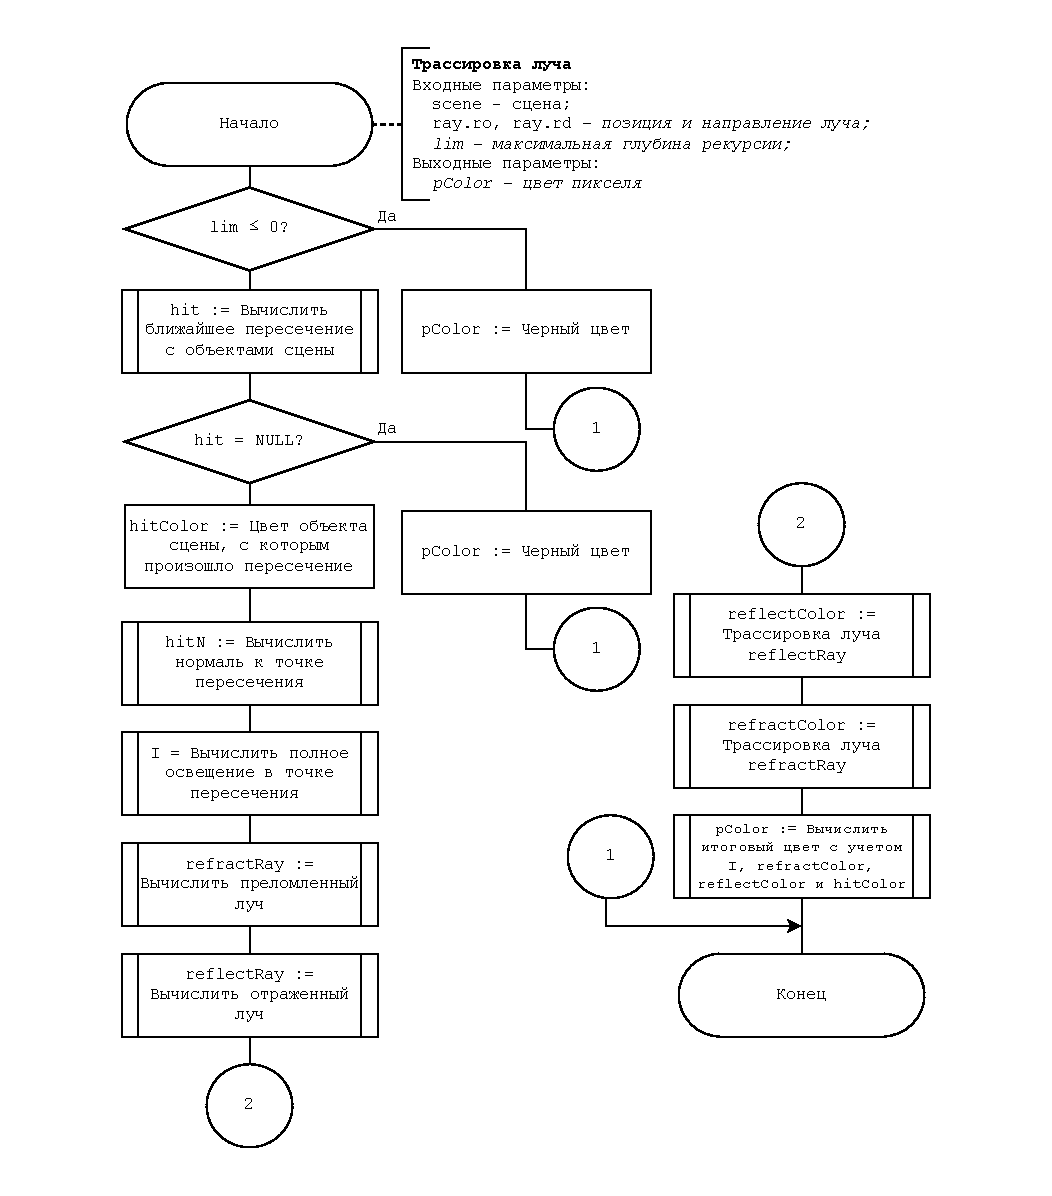
\includegraphics[scale=0.9]{diag/main-raytracing-pixel.pdf}
	\end{center}
	\caption{Схема алгоритма трассировки луча}
	\label{fig:pixel}
\end{figure}

На рисунке~\ref{fig:pixels} изображена схема алгоритма обратной трассировки лучей для вычисления цвета всех пикселей изображения.

\newpage
\begin{figure}[ht!]
	\begin{center}
		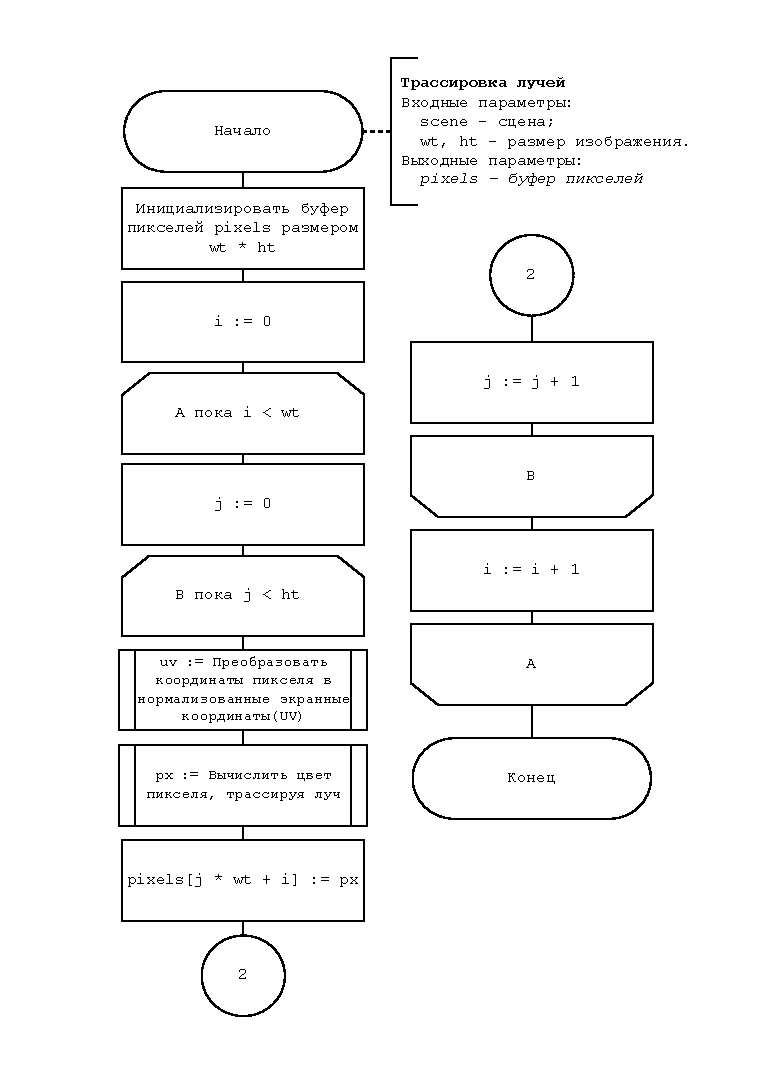
\includegraphics[scale=0.9]{diag/main-raytracing-pixels.pdf}
	\end{center}
	\caption{Схема алгоритма трассировки лучей}
	\label{fig:pixels}
\end{figure}

\subsubsection{Общий алгоритм работы программы}

На рисунке~\ref{fig:gen} представлена схема общего алгоритма работы программы.

\newpage
\begin{figure}[ht!]
	\begin{center}
		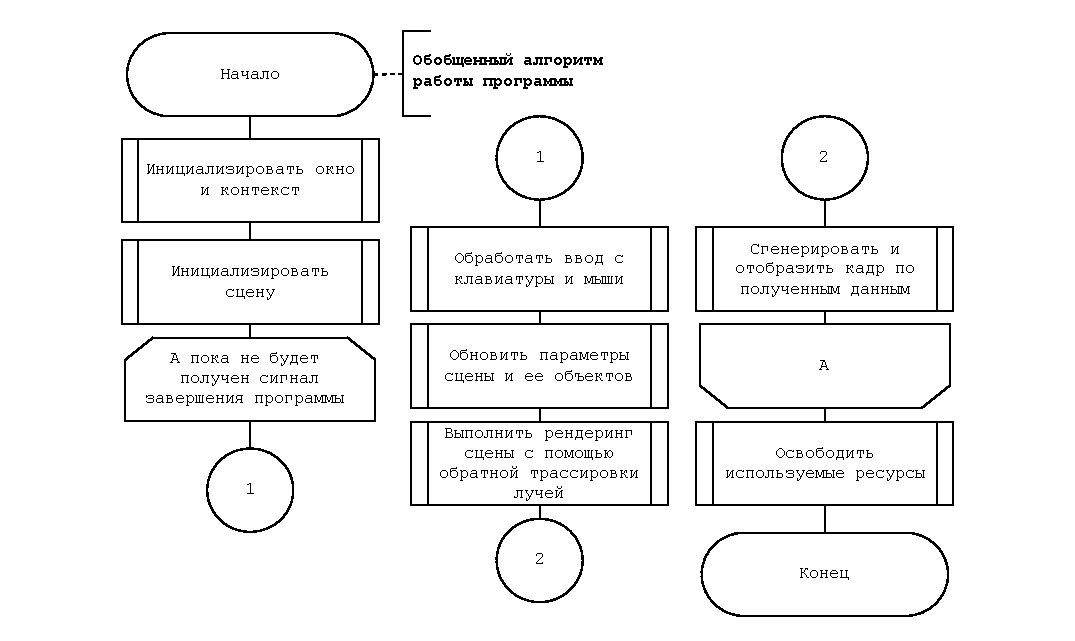
\includegraphics[scale=0.9]{diag/main-general.pdf}
	\end{center}
	\caption{Схема общего алгоритма работы программы}
	\label{fig:gen}
\end{figure}

\subsection{Используемые типы и структуры данных}

В таблице~\ref{tb:types-1} описаны используемые типы и структуры данных.

\begin{table}[ht!]
	\caption{Используемые типы и структуры данных (начало)}
	\centering\setstretch{1.5}	
	\begin{tabular}{|c|>{\arraybackslash}p{10.5cm}|} \hline
		\textbf{Объект} & \textbf{Представление / тип данных} \\
		\hline\hline
		
		\texttt{Трехмерный вектор} & Структура vec3 с полями: x, y, z -- числа с плавающей точкой. \\ \hline
		
		\texttt{Цвет} & Структура ColorRGB с полями: r, g, b -- числа с плавающей точкой. \\ \hline
		
		\texttt{Луч} & Структура Ray с полями orig и dir -- трехмерные векторы. \\ \hline
		
		\texttt{Источник света} &  Структура Light с полем pos -- трехмерный вектор. \\ \hline
	\end{tabular}\label{tb:types-1}
\end{table}

\newpage
\setcounter{table}{2}
\begin{table}[ht!]
	\centering\setstretch{1.5}	
	\caption{Используемые типы и структуры данных (окончание)}
	\begin{tabular}{|c|>{\arraybackslash}p{10.5cm}|} \hline
		\textbf{Объект} & \textbf{Представление / тип данных} \\
		\hline\hline
		
		\texttt{Камера} & Структура Camera с полями: pos -- трехмерный вектор; yaw, pitch, fov -- числа с плавающей точкой. \\ \hline
	
		\texttt{Тело} & Структура Shape c полями: pos (трехмерный вектор); color (цвет); reflect (коэффициент отражения света), refract (коэффициент пропускания света), n (коэффициент преломления света) -- числа с плавающей точкой. \\ \hline
		
		\texttt{Плоскость} & Структура Plane c полями структуры Shape и полем height -- число с плавающей точкой.\\ \hline
		
		\texttt{Цилиндр} & Структура Cylinder c полями структуры Shape и полями height, radius -- числа с плавающей точкой.\\ \hline
		
		\texttt{Параллелепипед} & Структура Box c полями структуры Shape и полями min, max -- трехмерные векторы.\\ \hline
		
		\texttt{Пересечение с объектом} & Структура RayHit c полями: pos, nrm -- трехмерные векторы; n -- число с плавающей точкой. \\ \hline
		
		\texttt{Сцена} & Структура Scene c полями: camera (камера), light (источник света), shapes (тела) -- массив структур Shape. \\ \hline
	\end{tabular}
\end{table}
	
\subsection*{Вывод}

В данном разделе были приведены функциональные требования к программному обеспечению, разработаны схемы алгоритмов, описаны типы и структуры данных, которые будут использованы при разработке.

